\subsection{Summary}
So far, we have studied the different ways to go through a kNN computation from a workflow point of view with three main steps.
The first step focuses on data preprocessing, and we review two main techniques. 
The first preprocessing technique, based on projecting the data to a one-dimension space, facilitates the next steps, because it is easier to manipulate 
data in one dimension rather than in high dimensions. 
However, data locality might not be preserved through this technique, and this is why, for a given set of initial data, several projections are performed 
with different seeds, to be able to spot errors. Consequently, the resulting dataset contains more data than the original one\footnote{The new data set is actually
the union of the data that arise from the different projections}.
The second preprocessing technique is not based on transforming the data but rather on selecting the data that are significant in the dataset, like the ones being in the middle of a cluster of data. To find those significant data, a sampling must be done on the initial dataset. This technique has no impact on the data itself.

The second step of the workflow focuses on data partitioning and organization in the partitions. 
%We reviewed two kinds of partitioning techniques: the 
%ones that are based on the distance between data and the one that are based on the size of the partition.
The distance based partitioning technique divides the data according to their distance with given reference points.
%The first kind of partitioning technique computes the distance of data to given references points, and assign them to the partition of 
%the closest 
%reference. 
This technique is straightforward although it does not guarantee finding the kNN in a single partition, because there is no bound on  the 
number of points in a given partition. 
The size based technique can address this problem by constructing partitions of a given size. However, there is no guarantee that all the kNN will be found in a given partition unless sophisticated schemes are used when creating the partitions.
During the partitioning step, data can also be organized using efficient data structures that offer good properties for searching and sorting.
% Such structured techniques come from solutions that have been introduced to compute efficiently a kNN on a single machine. Those techniques can be reuse unchanged in a given partition to 
%speed up a local computation.  


The last step of the workflow is to actually compute the kNN. This step can be done in one or two MapReduce jobs. Choosing one way or the other essentially depends on the number of distances that need to be sorted.

%Here two approaches exist. 
%In the first approach, the entire dataset $S$ is checked for a 
%given partition of the dataset $R$, so that the kNN computation can be done in a single MapReduce job. Of course, this supposes that the 
%entire dataset $S$ 
%is bearable for a single computing unit. \TODO{I don't agree. Only the distances have to fit in memory. With good partitioning it is entirely possible}.  In the second approach, both $S$ and $R$ are partitioned such that two MapReduce jobs are needed: one to compute 
%the local kNN and one to compute the final kNN among the local candidates. The advantage of this approach is that it is less computation intensive than 
%the first one, since not all data in $S$ are checked for a given data in $R$. However, the cost to trigger a second MapReduce job should not be neglected: 
%the first solution is probably more efficient when $|R|$ is large $|S|$ not so much. Here, a tradeoff between cost and gain of parallelization and 
%distribution must be made. \TODO{I don't agree, it does not match the execution section!}


Figure~\ref{workflow} summarizes the 
workflow we have gone through in this section and the techniques that are associated with each step. 
As those steps are more or 
less independent from each other, it is possible to focus on a particular step and  choose the 
technique that best fits  the use case, without 
impacting the next step. Hence it is possible to create a new kNN workflow by carefully selecting 
the algorithm at each step. For example, one can choose to transform the data with LSH or z-value in the pre-processing stage, then split them into blocks with Size Based Partitioning method, and use one or two rounds of MapReduce jobs for computation and sort.

%\TODO{we really need a convincing example here}.
%one could preprocess the data with LSH and then partition the data the advantage is that it is very efficient in the preprocessing phase if the bottleneck lies there

\begin{figure*}[t]
\center
\scalebox{0.35}{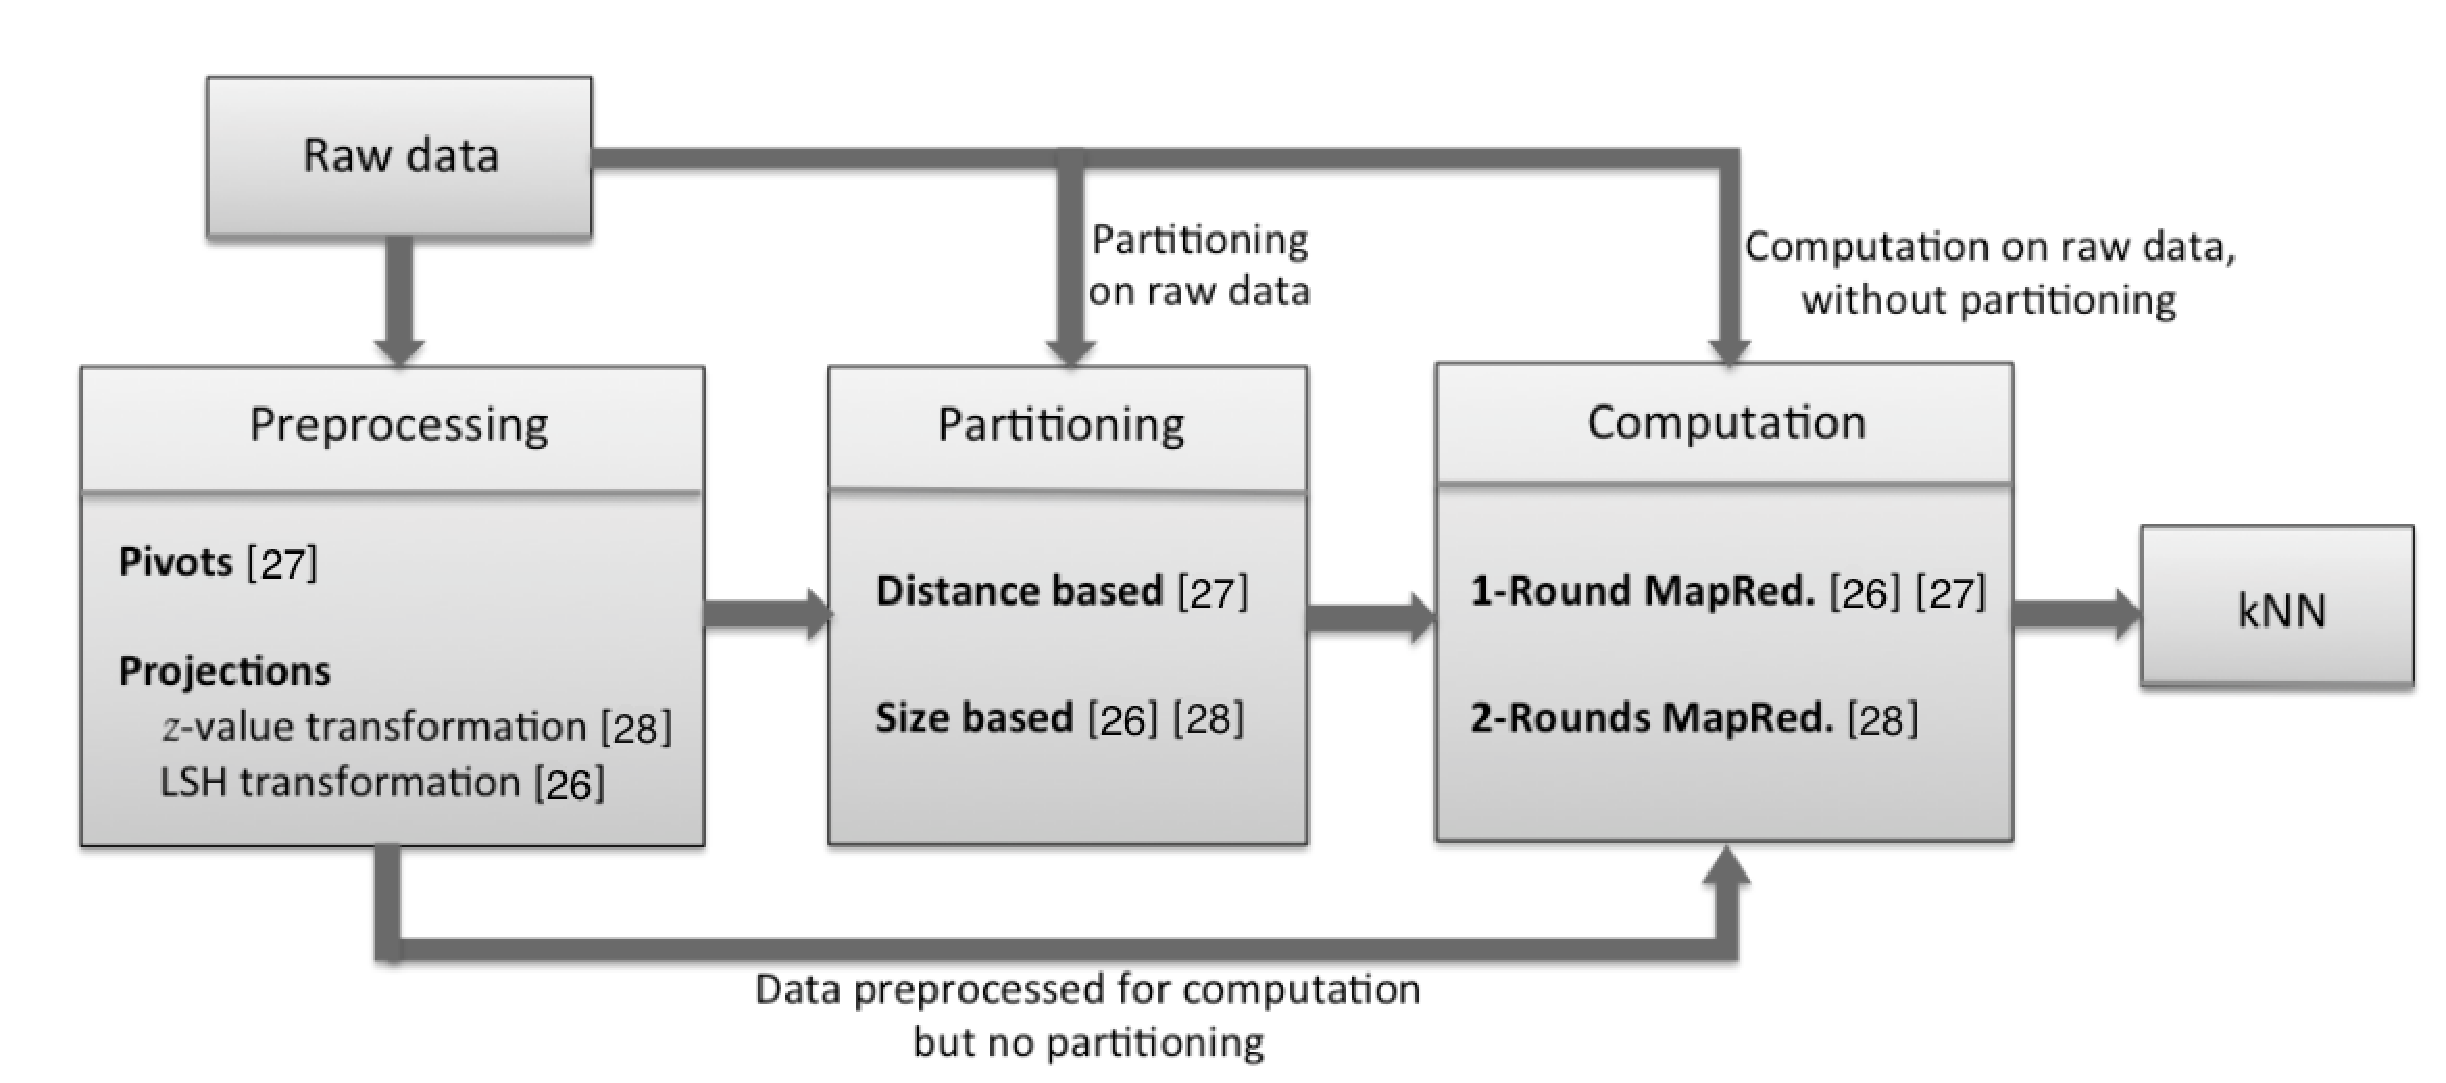
\includegraphics{res/workflow.pdf}}
\caption{Usual workflow of a kNN computation using MapReduce \label{workflow}}
\end{figure*}
